\chapter{Results}


\section{The effect of G3BP1 tethering on mRNA dynamics}

Proteins of the G3BP RNA-binding family have shown relevance in SGs.
In mammals, G3BP1 (and its paralog G3BP2) were reported to be essential in nucleating the formation of SGs \cite{kedersha_g3bp-caprin1-usp10_2016}.
SGs can not only be induced by stress (e.g. sodium arsenite) but also by the overexpression of G3BPs \cite{tourriere_rasgap-associated_2003}.
The exact role of G3BPs in SG assembly as well as in unstressed cells is still largely unknown.
As reviewed in Alam and Kenedy \cite{alam_rasputin_2019} various functions have been attributed to this protein family.
These range from transcript destabilization and repression to the polar opposite in transcript stabilization.
Furthermore, G3BP's also showed effects on transcript localization and sequestration to
    virus-induced foci.
The only consensus is G3BP's involvement in mRNA translational control.
The subsequent experiments attempt to clarify this disunity by analyzing G3BP1's effect on mRNA transcripts at a single-molecule level.

This study focussed on one reporter RNA containing a SunTag cassette, the gene encoding for \textit{Renilla} luciferase and MS2 stem-loops (Figure \ref{fig:mcp_images}A).
These stem-loops are structural motifs derived from phages and can be specifically recognized by a bacteriophage MS2 coat protein (MCP).
G3BP1 was fused to MCP (abbreviated as MCPG3) in an attempt to increase transcript level concentration and improve mRNA recruitment to SGs.
The construct was validated by FISH against the reporter RNA followed by immunofluorescence for the endogenous SG marker TIA-1 \cite{kedersha_rna-binding_1999} (Figure \ref{fig:mcp_images}B).
As a control, an identical construct only lacking G3BP1 fusion was used.
Both by visual inspection as well as by mRNA quantification (Figure \ref{fig:mcp_images}C), a significant difference in SG association can be seen.
MCPG3 shows an around two-fold increase in SG associated mRNAs compared to the control.
Taken together, fusing G3BP1 to MCP seems to be a reliable way to recruit functional G3BP1 to the local vicinity of mRNAs.

\begin{figure}[h]
    \centering
    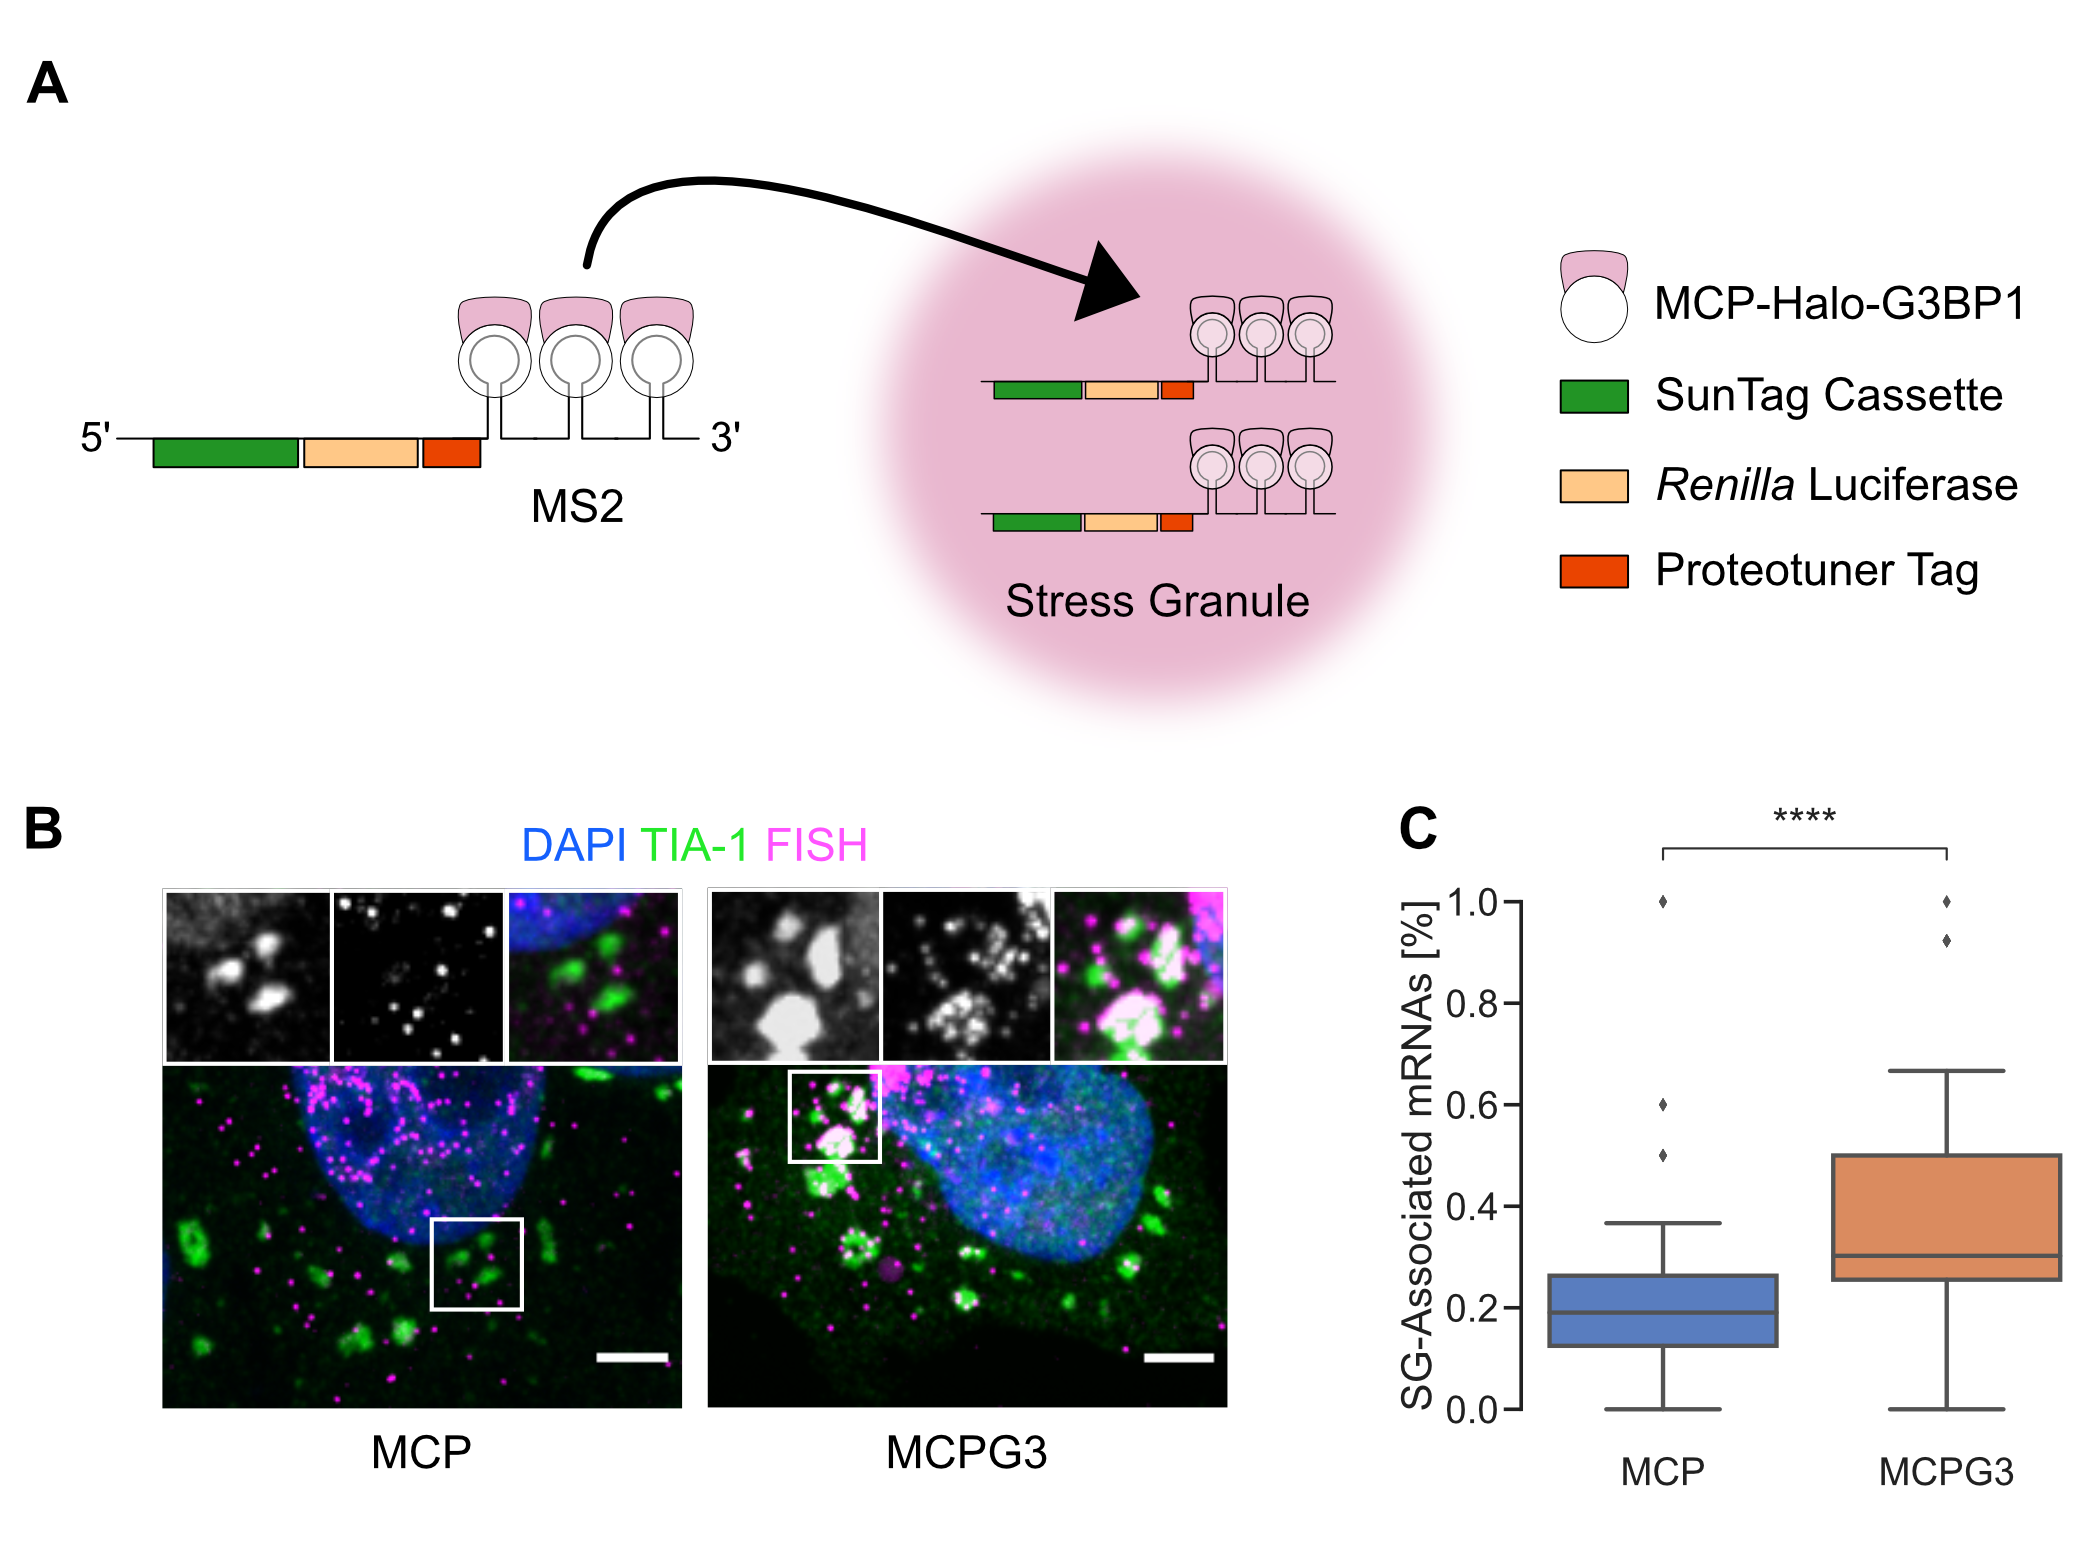
\includegraphics[width=\linewidth]{images/figure2}
    \caption{\textbf{Design of MCP-G3BP1.}
        (A) Schematic depiction of MCP-G3BP1 function.
        (B) Representative fluorescence images of the SG marker
            TIA-1 and the tethered RNAs.
            Pannels show TIA-1, FISH, Merge respectively.
            Scale bars, 10 \textmu m.
        (C) Quantification of the mRNA recruitment to SGs.
            Number of cells quantified (left to right): 27, 21. 
    }
    \label{fig:mcp_images}
\end{figure}

\subsection{Global translational activity} \label{mcp_luciferase}

Having proven that G3BP1 can be recruited to mRNAs,
    I wanted to investigate the effect on translational activity.
\textit{Renilla} luciferase assays are used to measure reporter expression on a global level.
As G3BP1 was shown to be involved in stress-induced events as well as in unstressed conditions,
    time points during both induction and stress recovery were measured.

MCPG3 showed a significant increase in luciferase readings in both induction and stress recovery (Figures \ref{fig:mcp_luciferase}A and \ref{fig:mcp_luciferase}B).
Interestingly, the largest effects are at later time points and not immediately after stress recovery.
This suggests a lesser involvement of G3BP1 on translational activity during stress.
SGs have been observed to persist between a few minutes to hours \cite{chen_relationships_2017}.
It is around this time that an increase in luciferase activity can be observed again.

\begin{figure}[h]
    \centering
    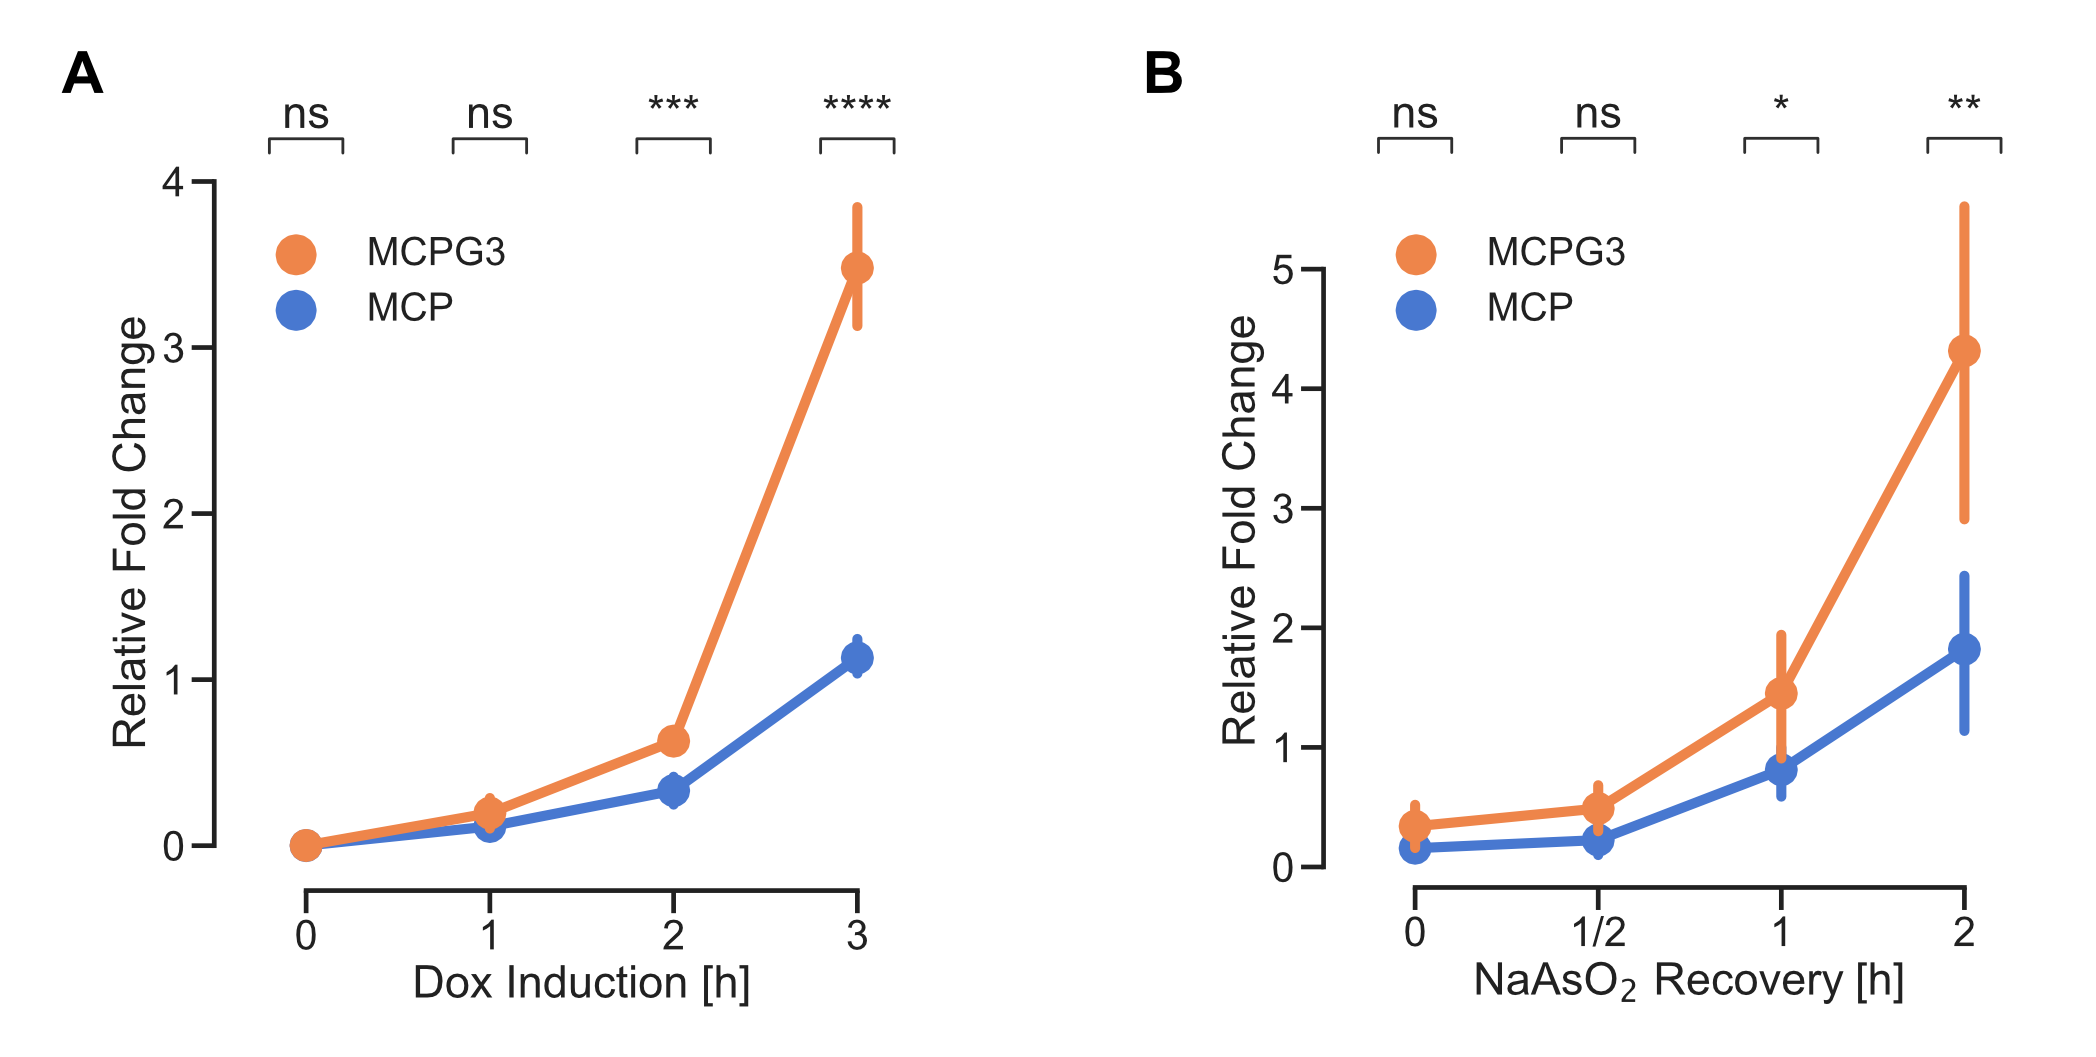
\includegraphics[width=\linewidth]{images/figure3}
    \caption{\textbf{G3BP1 tethering increases global translational activity.}
        (A) Luciferase assays at different time points during induction.
        (B) Sodium arsenite stress recovery time points after induction.
        (A and B) Data normalized to the 3 hour induction condition of MCP.     
    }
    \label{fig:mcp_luciferase}
\end{figure}

\subsection{Transcript level activity}\label{mcp_suntag}

The observed differences in luciferase activity described in Section \ref{mcp_luciferase} can result from various causes.
These translational differences could arrive by an increase in translational activity.
The translation site imaging method SunTag (see Section \ref{translation_site_imaging}) can be used to address this option.

In SunTag, the fluorescence intensity is a direct measure of protein production.
Therefore, to analyze the translation activity of MCPG3, the track intensity was quantified.
Track intensity refers to the average fluorescence intensity over the entire track duration.

During stress conditions, most mRNAs get translationally silenced (reviewed in Holcik and Sonenberg \cite{holcik_translational_2005}).
In order to image translation sites despite this silencing, images were acquired 15 to 30 minutes after removing the stressor.

Analysis of track intensity across entire images shows similar fluorescence intensities (Figure \ref{fig:mcp_suntag}A).
As was to be expected, the translational silencing during stress is not fully recovered leading to lower readings in the recovering cells.
Equivalently to the image-level analysis, cellular intensities (Figure \ref{fig:mcp_suntag}B) do not yield different results.
Similarly, the average intensity of all tracks per cell does not appear to be affected by G3BP1 fusion.

Lastly, global translation can also increase by a higher number of translating transcripts per cell.
However, as is evident from Figure \ref{fig:mcp_suntag}C the number of tracks stays consistent in all experiments.
This concludes that G3BP1 does not have a profound impact on translation activity.

\begin{figure}[H]
    \centering
    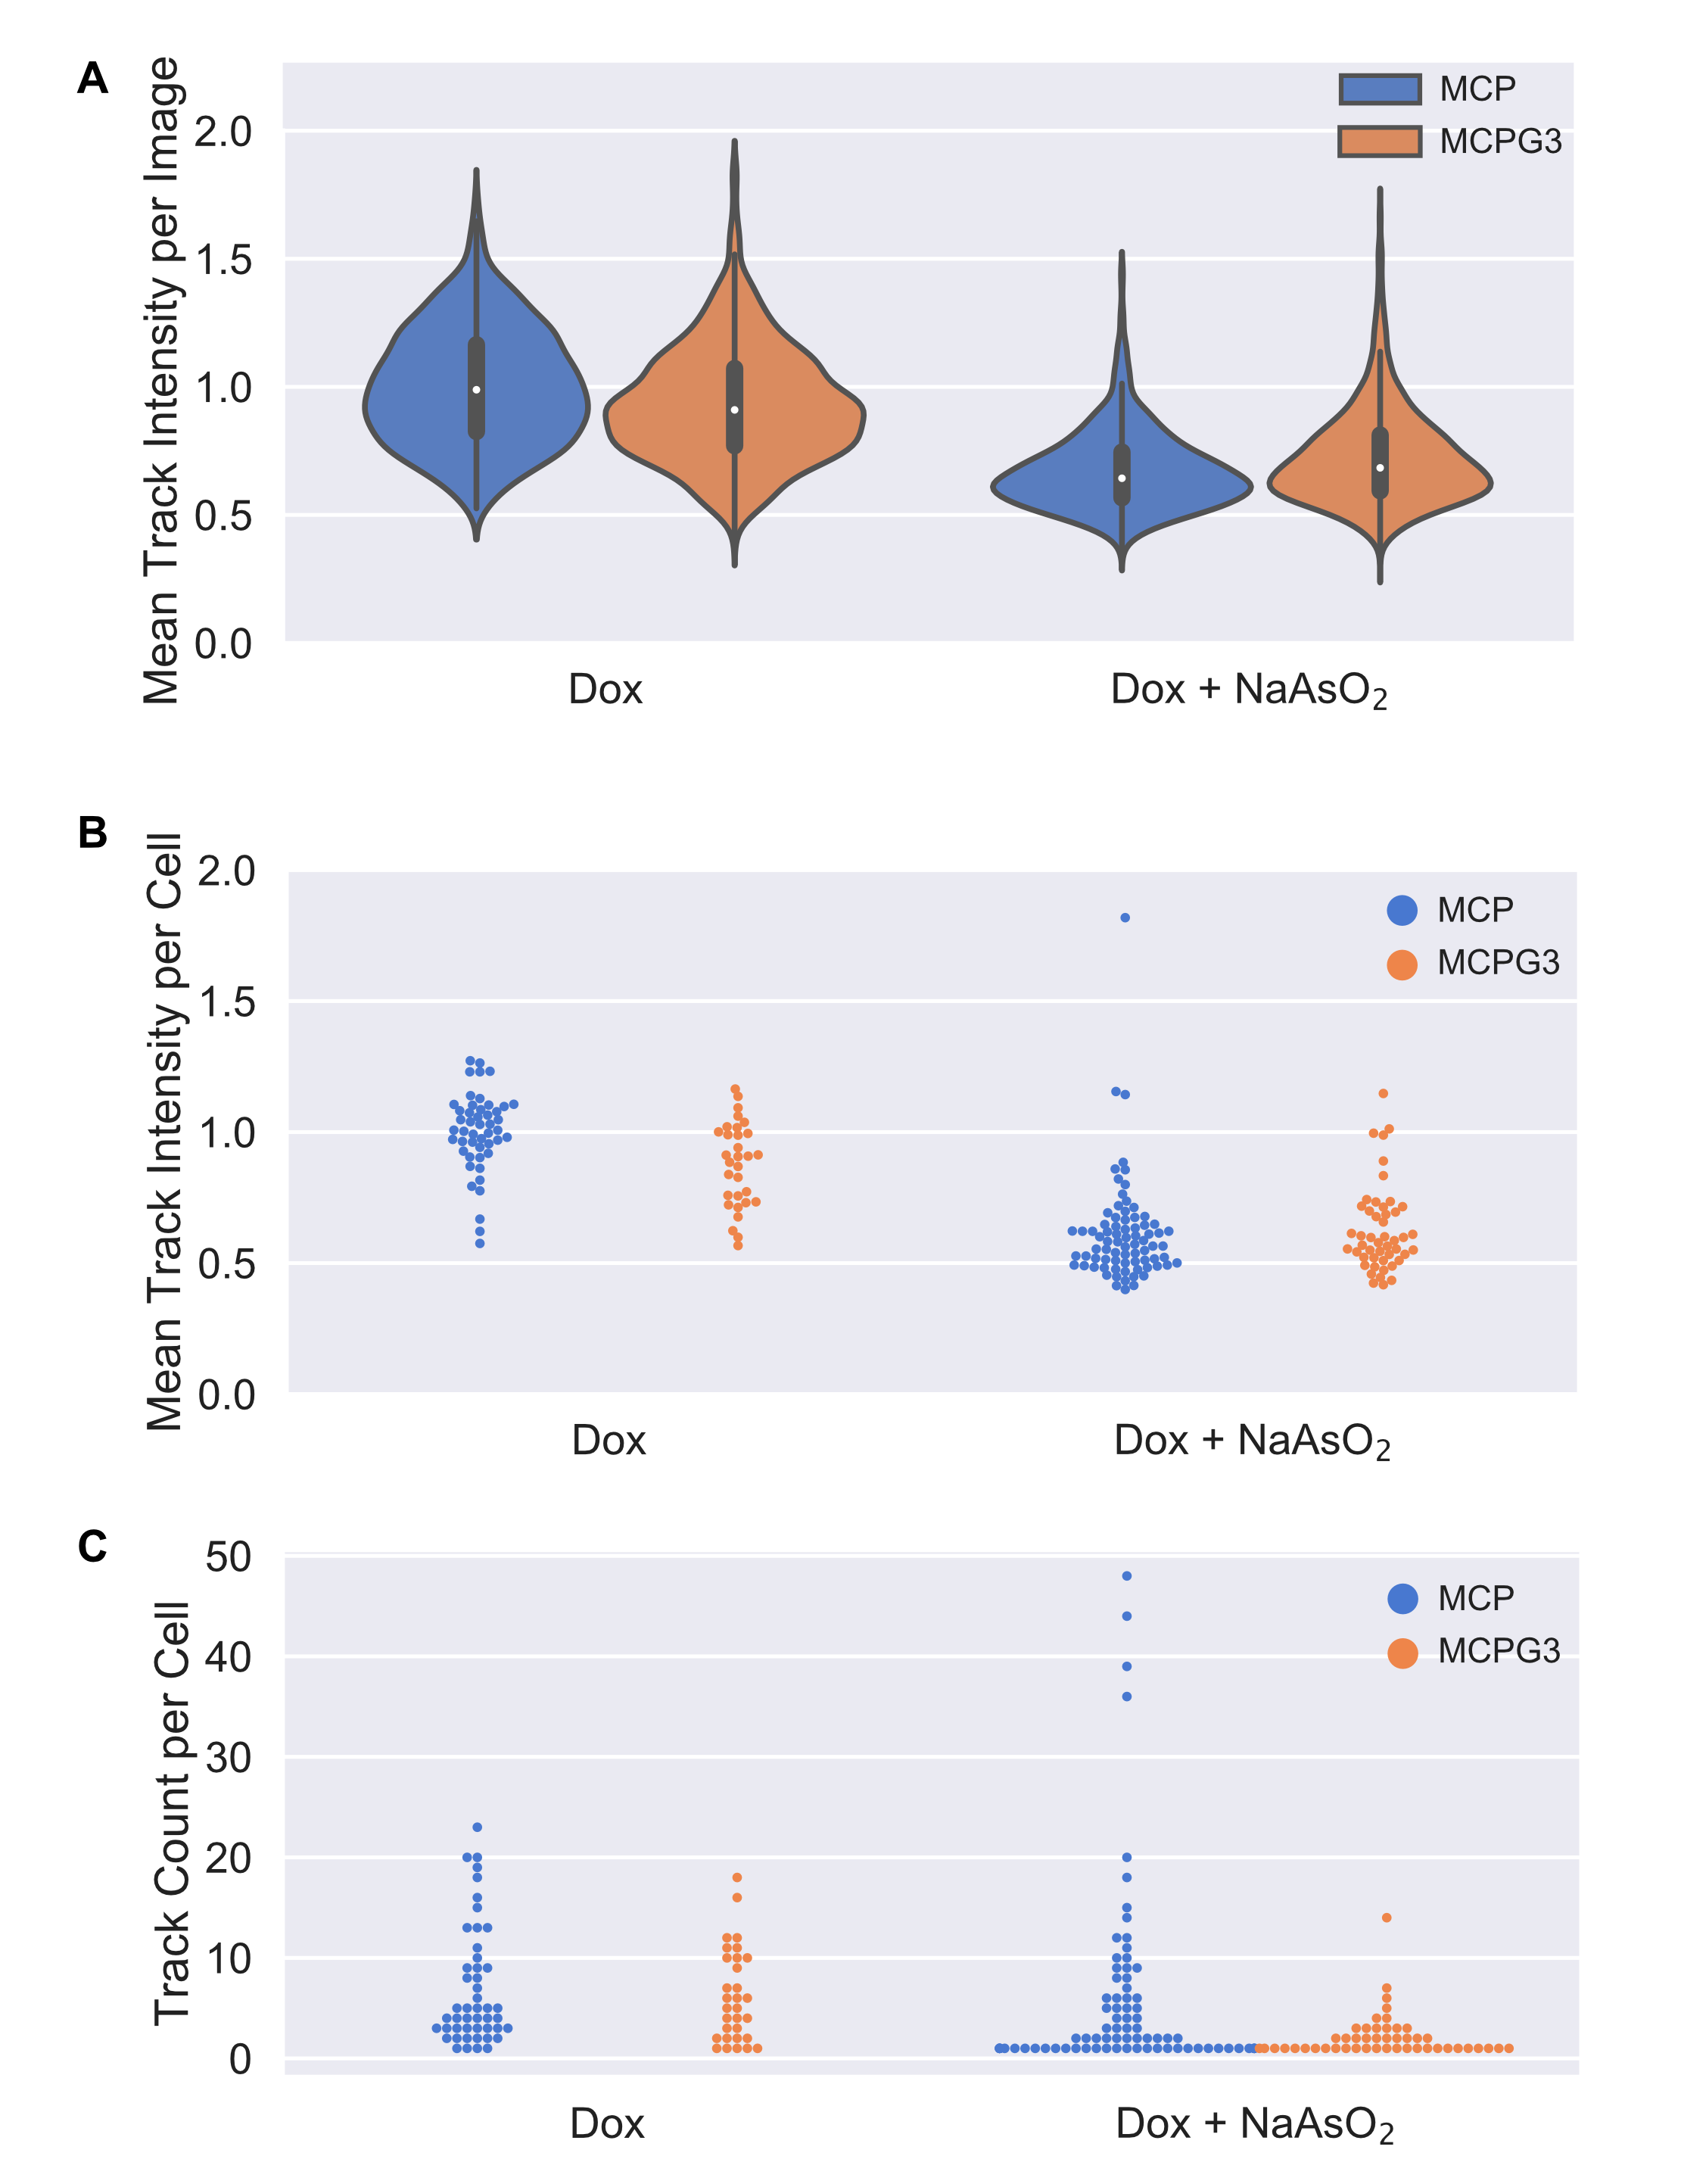
\includegraphics[width=\linewidth]{images/figure4}
    \caption{(Continued on the following page.)}
    \label{fig:mcp_suntag}
    \end{figure}
    \addtocounter{figure}{-1}
    \begin{figure} [t!]
    \caption{\textbf{Transcript level imaging of mRNAs.}
        (A) Distribution of the mean fluorescence intensity of tracked
            mRNAs in the full-sized image (without cellular segmentation).
            The total number of tracks (left to right): 715, 1064, 997, 3442.
        (B) Track intensity averaged per cell.
        (A and B) Data normalized to the Dox induction condition for MCP.
        (C) The number of tracks registered per cell.
        (B and C) The total number of cells (left to right): 48, 77, 31, 48.
    }
\end{figure}

\subsection{Transcript level stability} \label{mcp_treat}

SunTag measurements (see Section \ref{mcp_suntag}) did not suggest any effect of G3BP1 on translational activity.
Alternatively, a decrease in mRNA degradation could also explain the original luciferase readings.
To ask whether G3BP1 has an mRNA stabilizing effect, I compared the number of intact transcripts between MCPG3 and the control using 3(three)'-RNA end accumulation during turnover (TREAT) \cite{horvathova_dynamics_2017}.

TREAT uses a slightly modified reporter mRNA containing viral RNA pseudo-knot (PK) structures upstream of the MS2 stem-loops.
These PKs can block Xrn1 mediated 5'-3' degradation of a transcript by sequestering the 5' phosphate group \cite{kieft_new_2015}.
Subsequently, by using FISH probes against \textit{Renilla} luciferase upstream of PKs (showing intact mRNAs) and
    FISH probes against MS2 stem-loops downstream of PKs (showing both intact and degraded mRNAs) one can
    quantify the number of intact transcripts.

To look at transcript stabilization, five time points were chosen after induction followed by thorough washing to halt any further transcription.
As can be seen in Figure \ref{fig:mcp_treat}A, transcripts get exported to the cytosol as soon as transcription is stopped.

When comparing the percentage of intact mRNAs, i.e. transcripts still containing FISH spots 
    against both \textit{Renilla} luciferase and MS2, between MCPG3 and the control, a striking difference is evident (Figure \ref{fig:mcp_treat}B).
The G3BP1 fusion shows a significant increase in intact transcripts compared to the control suggesting an
    increase in mRNA stability.


\begin{figure}[h]
    \centering
    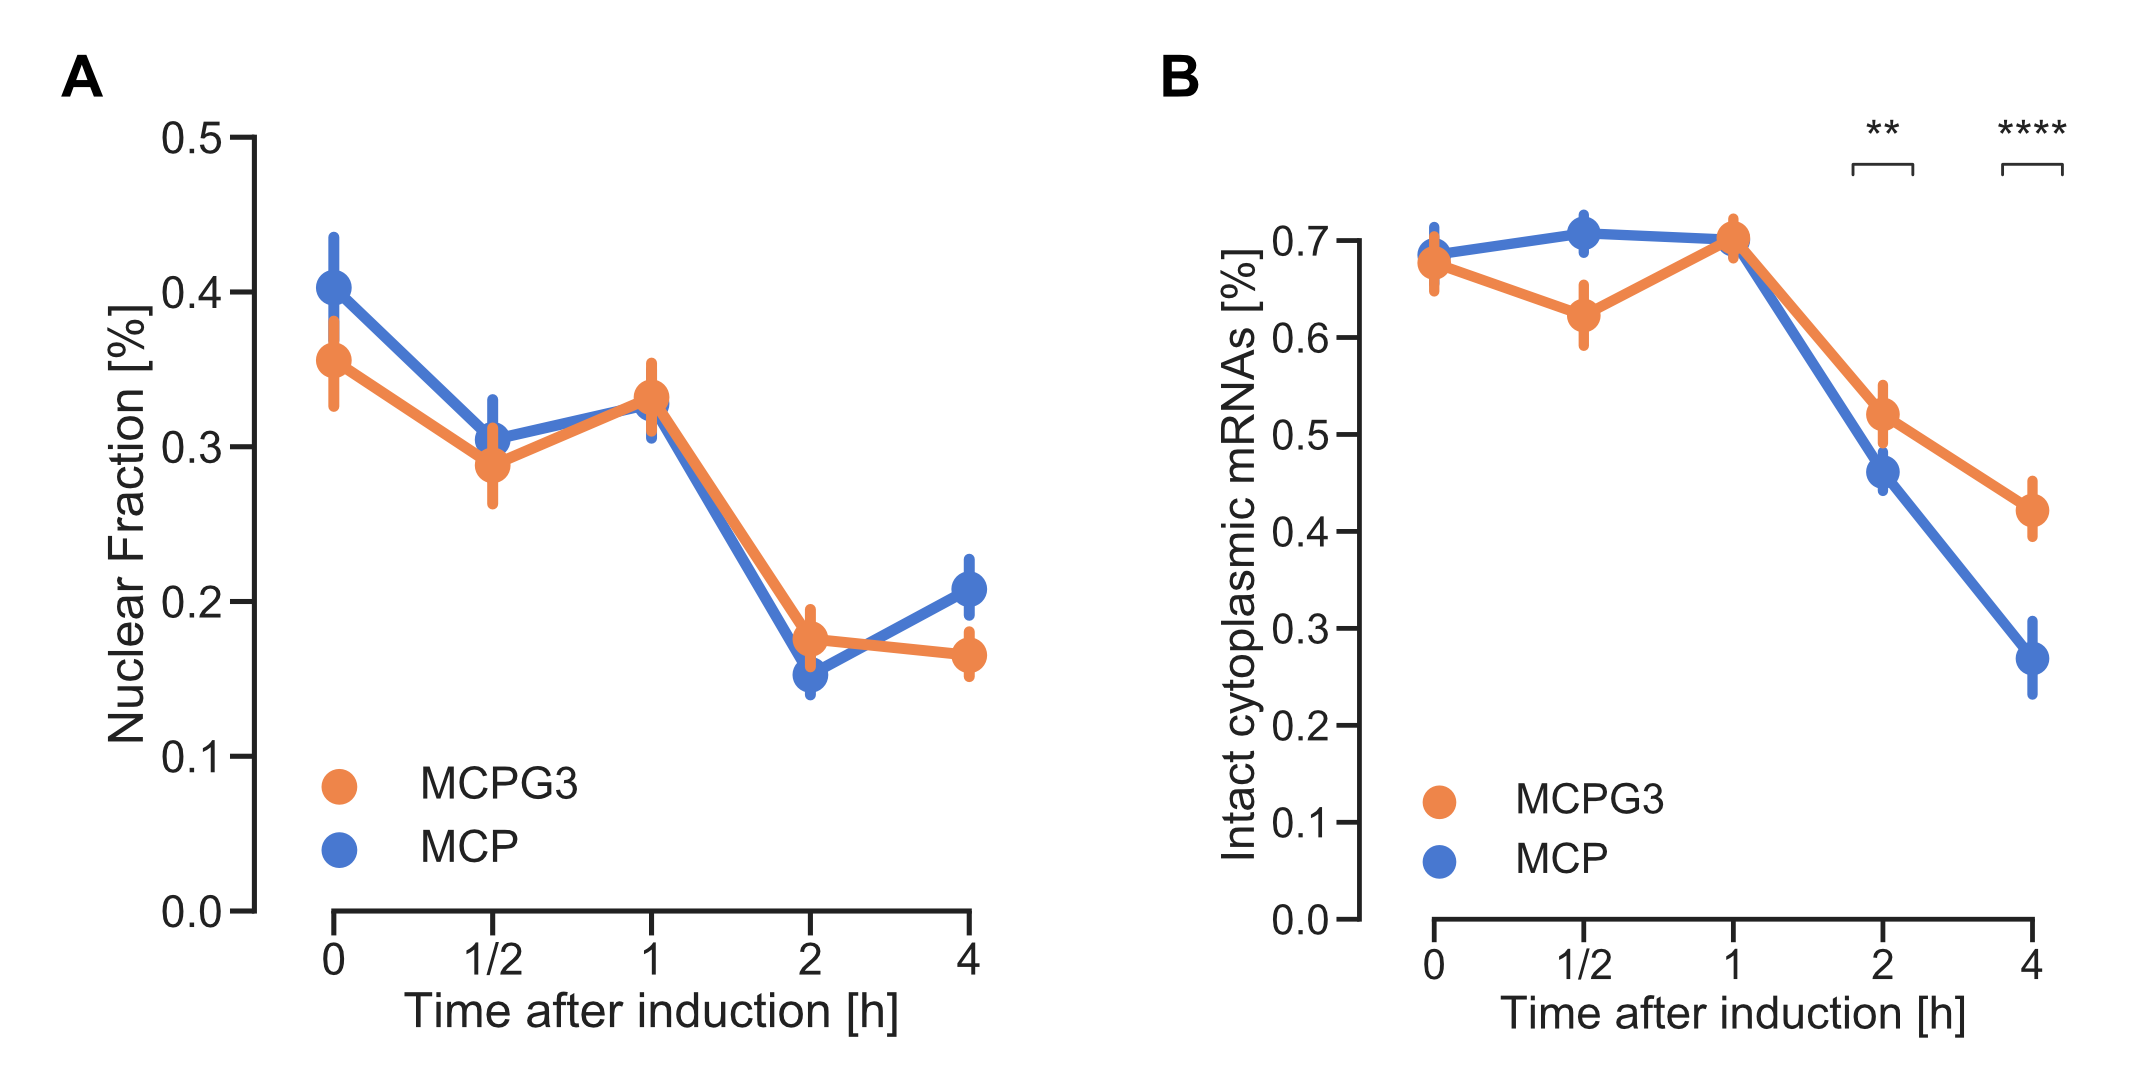
\includegraphics[width=\linewidth]{images/figure5}
    \caption{\textbf{TREAT based mRNA stability assay.}
        (A) The fraction of nuclear mRNAs (of total cellular mRNAs)
            at different time points after induction.
        (B) Percentage of intact cytoplasmic mRNAs at different time points.
        (A and B) Number of cells quantified (ascending, MCP then MCPG3):
            117, 154, 200, 175, 55, 114, 148, 167, 111, 132.
    }
    \label{fig:mcp_treat}
\end{figure}

\section{Improving the SunTag reporter}

The original design of the SunTag cassette consists of 24 GCN4 repeats.
These completely disordered repeats are thought to aggregate and could lead to a decrease in translation rates.
In an attempt to decrease protein disorder, a spaghetti monster reporter was made.
Spaghetti monster green fluorescent proteins (smGFP) are essentially a non-fluorescent green
    fluorescent protein's (GFP) beta-barrel used to attach small epitope tags.
Here, three GCN4 repeats each were placed at the N-terminus, C-terminus, and 10/11-loop of the GFP
    beta-barrel as shown in Figure \ref{fig:spaghetti}A.
Previously, other tags, such as influenza hemagglutinin (HA), were used and visualized with
    frankenbodies (single-chain antibodies targeting various tags) \cite{zhao_genetically_2019}.
To my knowledge, this is the first attempt to combine SunTag imaging with smGFP constructs.

Initially, it was of interest to see whether the smGFP reporter has higher translational activity.
As is evident from Figure \ref{fig:spaghetti}B, the new reporter shows an approximative 4-fold
    increase in luciferase activity.
A pure \textit{Renilla} reporter was used as control which does not contain any GCN4 repeats.
While the smGFP reporter drastically increases activity, it does not yet reach the levels
    of the control.
It must be noted, that the control construct does not contain an FKBP tag which has lowered
    the activity in previous experiments.

To look at the effect of the new reporter in live cells, stable cell lines were created and
    observed after 1 hour of induction.
From a representative image in Figure \ref{fig:spaghetti}C, one can see that cells typically
    have more, slightly dimmer translation sites.
Quantification of images showed a significant increase in the number of translation sites per cell (Figure \ref{fig:spaghetti}D).
The brightness of individual spots decreased around 2.7 fold (Figure \ref{fig:spaghetti}E).
This decrease can be explained by a lower number of GCN4 repeats available for the scAB to bind.
Whereas the standard SunTag has 24 GCN4 repeats, smGFP only has 9 leading to a binding site
    difference of 2.6$\overline{\mbox{6}}$ to 1.

Taken together, this study proposes a new SunTag reporter which increases translational activity
    by greatly increasing the number of active transcription sites.


\begin{figure}[h]
    \centering
    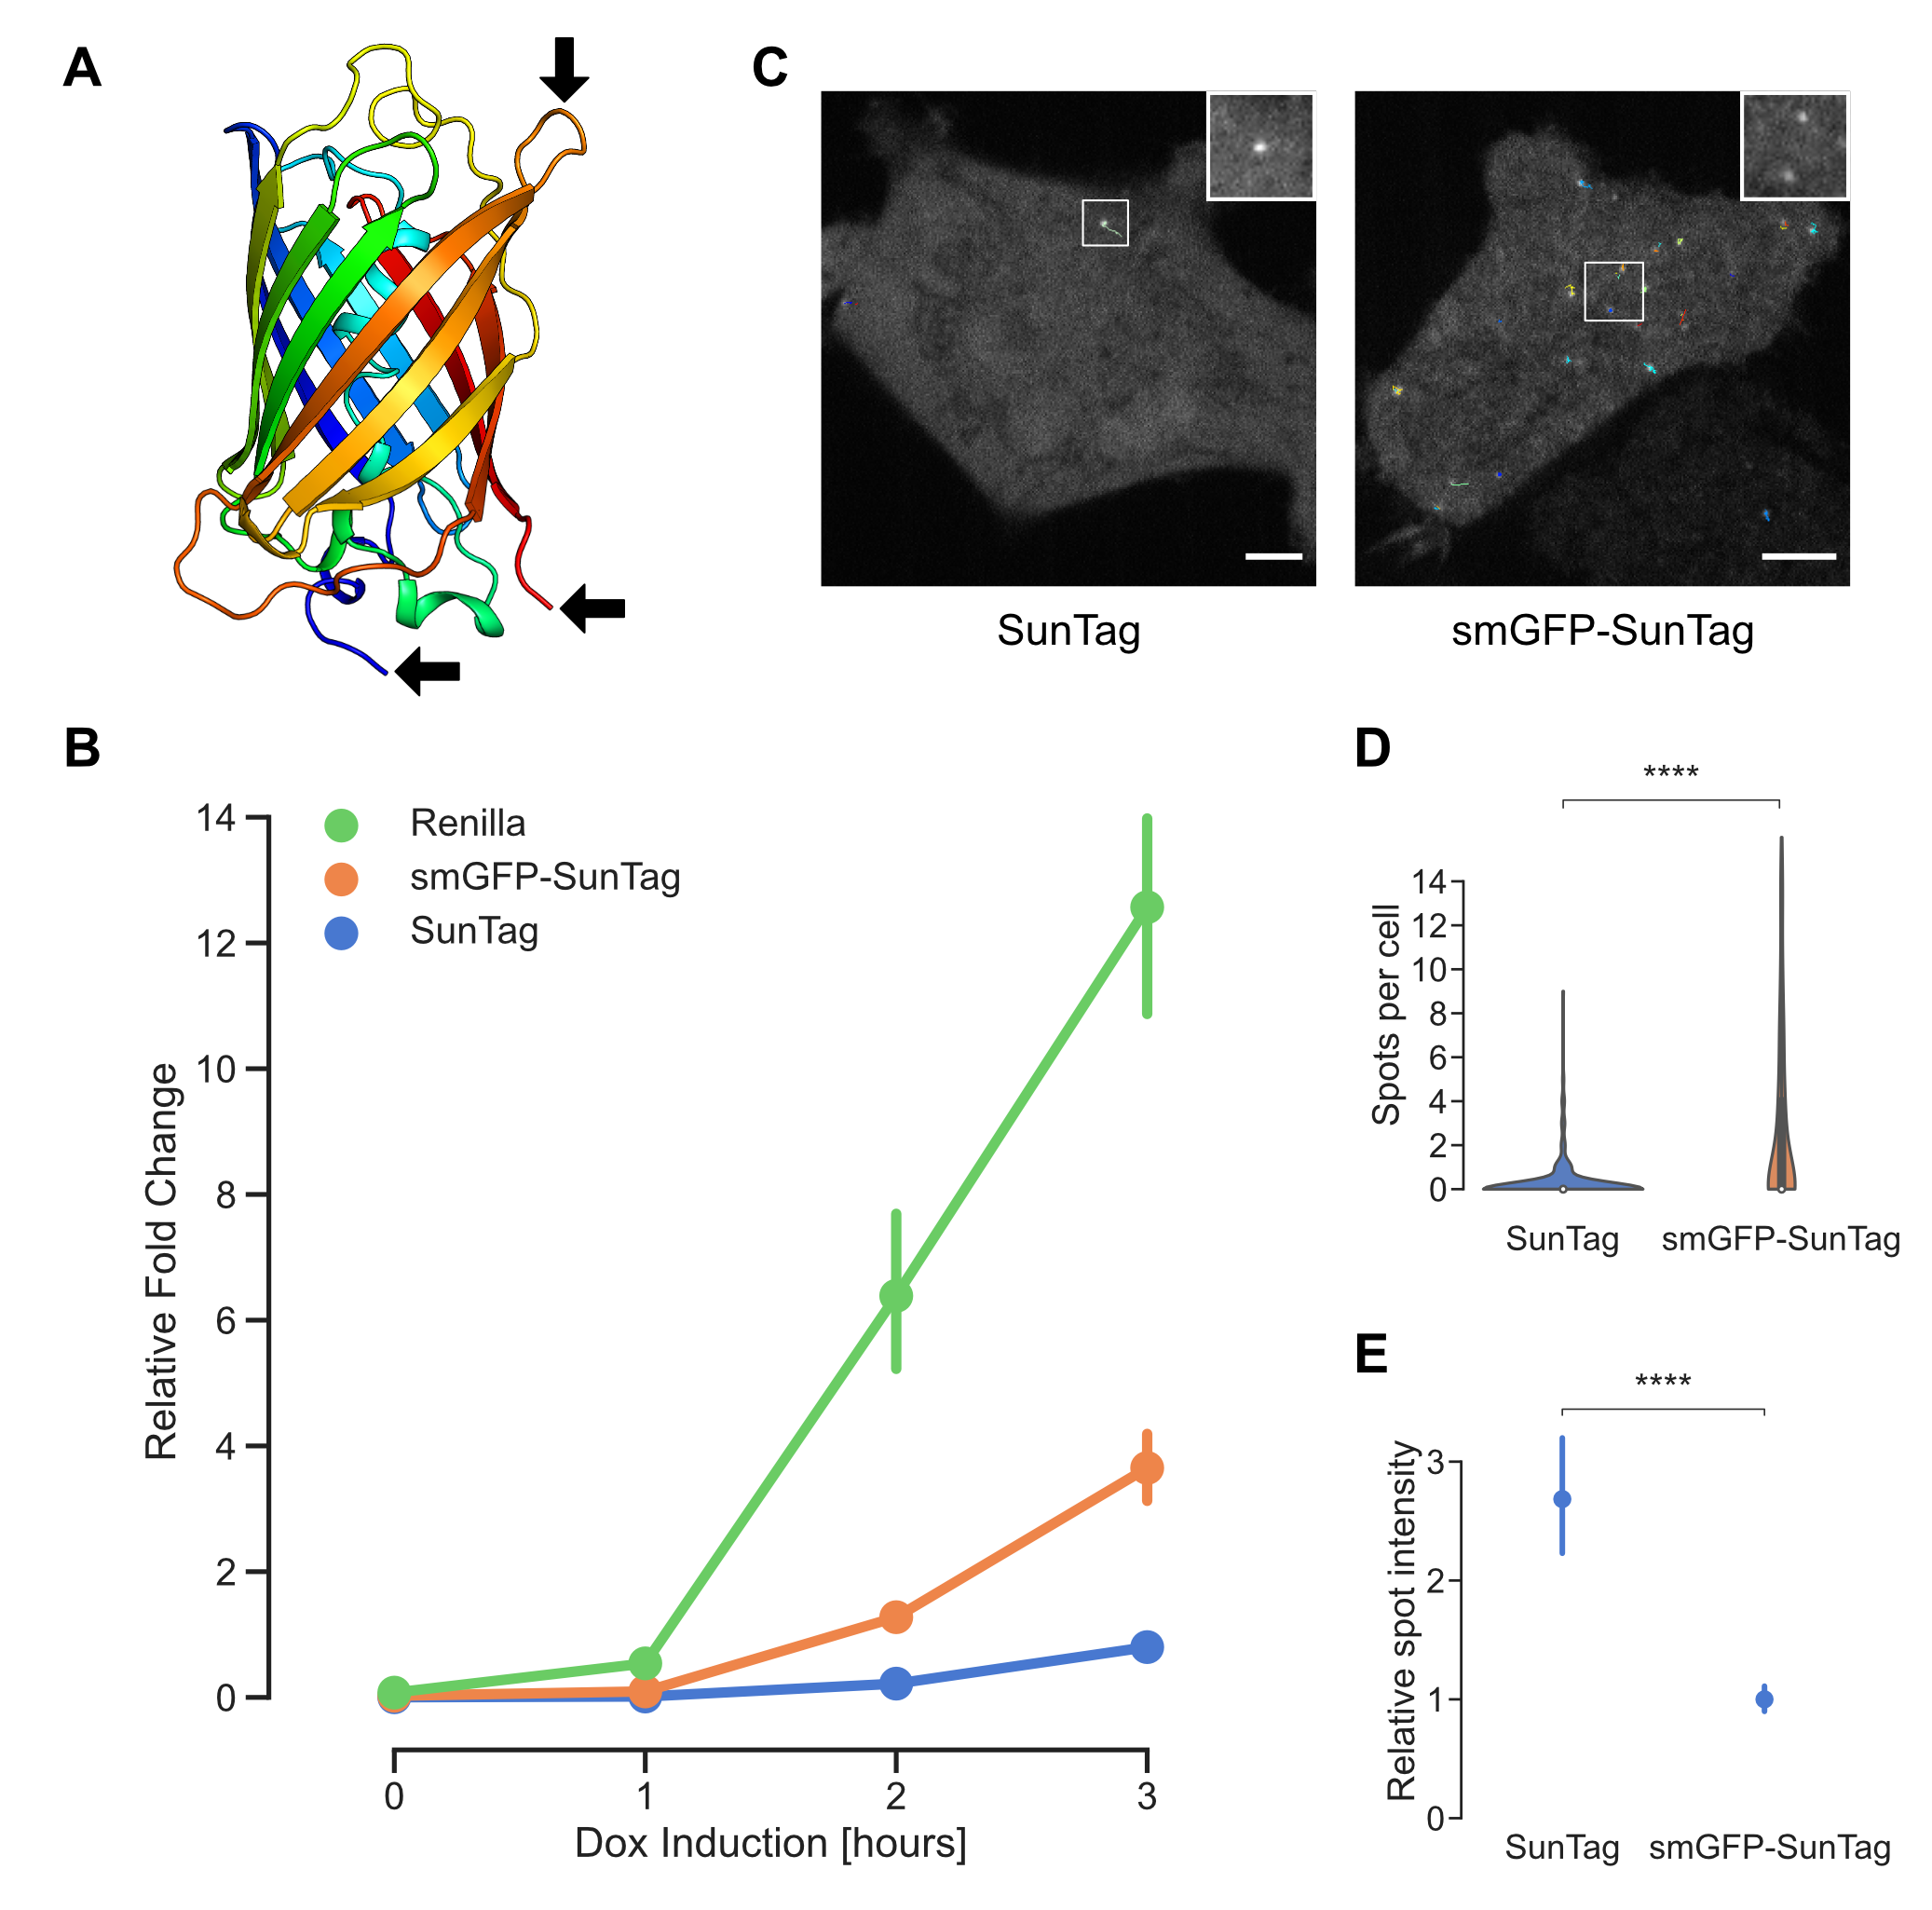
\includegraphics[width=\linewidth]{images/figure6}
    \caption{\textbf{Overview of the smGFP SunTag reporter.}
        (A) Structural overview of GCN4 repeat placement on the smGFP beta-barrel (PDB ID: 1GFL \cite{yang_molecular_1996}).
        (B) Relative luciferase activity comparing the standard SunTag reporter,
            the smGFP SunTag reporter, and a Renilla reporter without SunTag cassette.
        (C) Representative fluorescence images. Each recorded mRNA track is 
            visualized with a unique color. Scale bar, 10 \textmu m.
            The inset shows spots from raw images without brightness corrections.
        (D) Quantification of translation site count per cell.
            The number of cells quantified (left to right): 286, 233.
        (E) Average spot intensity normalized to the smGFP reporter.
            The number of spots quantified (left to right): 36, 39.
    }
    \label{fig:spaghetti}
\end{figure}